\documentclass[11pt]{article}

\usepackage[margin=1in]{geometry}
\usepackage{amsmath, amssymb}
\usepackage{graphicx}
\usepackage{booktabs}
\usepackage[hidelinks]{hyperref}

\title{Homework 2\\Network Dynamics and Learning}
\author{Alessandro Casadei}
\date{}

\begin{document}

\maketitle

\section{Introduction}

This homework studies continuous-time random walks and opinion dynamics on
directed networks. The first part considers a single-particle
continuous-time Markov chain, compares Monte Carlo estimates with theoretical
return and hitting times, and analyzes continuous-time French-DeGroot opinion
dynamics on the same weighted graph. The second part extends the random walk
model to many independent particles and compares the node-count simulation
with the stationary distribution predicted by the single-particle chain. The
third part studies open particle networks with external arrivals, comparing
proportional service rates with fixed service rates.

The workflow combines Monte Carlo simulation, direct theoretical computation,
comparison between simulation and theory, and stability analysis. All reported
numerical values are taken from the saved result files or from formulas
applied to the same model parameters. The report uses the same row-source,
column-destination convention as the code and the saved CSV files.

\section{Problem 1 --- Single-particle continuous-time random walk and French-DeGroot dynamics}

\subsection*{Model definition}

The node order is fixed as
\[
    [o,a,b,c,d].
\]
The closed-network rate matrix is
\[
\Lambda =
\begin{pmatrix}
0 & 2/5 & 1/5 & 0 & 0\\
0 & 0 & 3/4 & 1/4 & 0\\
1/2 & 0 & 0 & 1/3 & 0\\
0 & 0 & 1/3 & 0 & 2/3\\
0 & 1/3 & 0 & 1/3 & 0
\end{pmatrix}.
\]
The convention is that $\Lambda_{ij}$ is the transition rate or edge weight from
node $i$ to node $j$, so rows are source nodes and columns are destination
nodes. Let
\[
    \omega = \Lambda \mathbf{1}, \qquad
    Q = \Lambda - \operatorname{diag}(\omega).
\]
Explicitly, the closed-network departure-rate vector is
\[
\omega=\Lambda\mathbf{1}
=
\left(\frac{3}{5},\,1,\,\frac{5}{6},\,1,\,\frac{2}{3}\right).
\]
Thus $\omega_i$ is the total rate at which the continuous-time Markov chain
leaves node $i$, and $Q$ is the generator. When the process is at node~$i$,
the holding time has mean $1/\omega_i$, and the next visited node is sampled
from the normalized row $\Lambda_{ij}/\omega_i$.

\subsection*{Parts (a)--(b): return time to node $a$}

The return-time simulation starts the particle at node $a$. I use the convention
that the initial holding time in $a$ is included: the clock starts immediately
at $a$, the first holding time in $a$ is sampled, and the stopping time is the
next entrance to $a$ after the particle has left. The simulation used 100000
Monte Carlo runs with seed 20260615.

The simulated mean return time was
\[
    \widehat{\mathbb{E}}_a[T_a^+] = 6.69375284456,
\]
with sample standard deviation $4.9131262948$, standard error
$0.0155366695236$, and 95 percent confidence interval
$[6.66330097229,\,6.72420471683]$.

For the theoretical value I used the CTMC stationary-cycle identity
\[
    \mathbb{E}_a[T_a^+] = \frac{1}{\pi_a \omega_a},
\]
where $\pi$ is the stationary distribution of the CTMC and the convention again
includes the initial holding time.
The factor~$\omega_a$ appears because this is a continuous-time return time.
In stationarity, the fraction of time spent in node~$a$ is~$\pi_a$, and while
the process is in~$a$, departures occur at rate~$\omega_a$.  Hence the
long-run rate of cycles from one entrance into~$a$ to the next one is
$\pi_a\omega_a$, and the mean cycle length is $1/(\pi_a\omega_a)$.
This convention includes the initial holding time in~$a$, consistently with
the simulation.
This gives
\[
    \mathbb{E}_a[T_a^+] = 6.7083.
\]
The simulation minus theory difference is $-0.0146$, corresponding to
a relative error of $-0.0022$. The theoretical value lies inside the
Monte Carlo confidence interval, so the two values agree up to sampling error.

\subsection*{Parts (c)--(d): hitting time from $o$ to $d$}

For the hitting-time simulation, the particle starts at node $o$ and the
simulation stops at the first visit to node $d$. The simulation used 100000
Monte Carlo runs with seed 20260616. The simulated average hitting time was
\[
    \widehat{\mathbb{E}}_o[T_d] = 10.7608365852,
\]
with standard deviation $8.94426026682$, standard error $0.0282842344285$, and
95 percent confidence interval $[10.7053994857,\,10.8162736847]$.

The theoretical hitting times $h_i=\mathbb{E}_i[T_d]$ solve
\[
    h_d = 0, \qquad
    \sum_j Q_{ij}h_j = -1 \quad \text{for } i \neq d.
\]
Solving this linear system gives
\[
    \mathbb{E}_o[T_d] = 10.7666666667.
\]
The simulation minus theory difference is $-0.00583008148547$, with relative
error $-0.000541493636421$, which is small compared with the Monte Carlo
standard error.

\subsection*{Part (e): French-DeGroot dynamics on the original graph}

I interpret $\Lambda$ as the weighted adjacency matrix of a directed graph and
use the continuous-time French-DeGroot model
\[
    \dot{x}(t) = -Lx(t), \qquad
    L = \operatorname{diag}(\Lambda\mathbf{1})-\Lambda.
\]
The representative trajectory in Figure~\ref{fig:p1-fdg-original} uses the
initial condition
\[
    x(0) = (1,\,-0.5,\,2,\,0.25,\,1.5),
\]
in the node order $[o,a,b,c,d]$.

\begin{figure}[htbp]
    \centering
    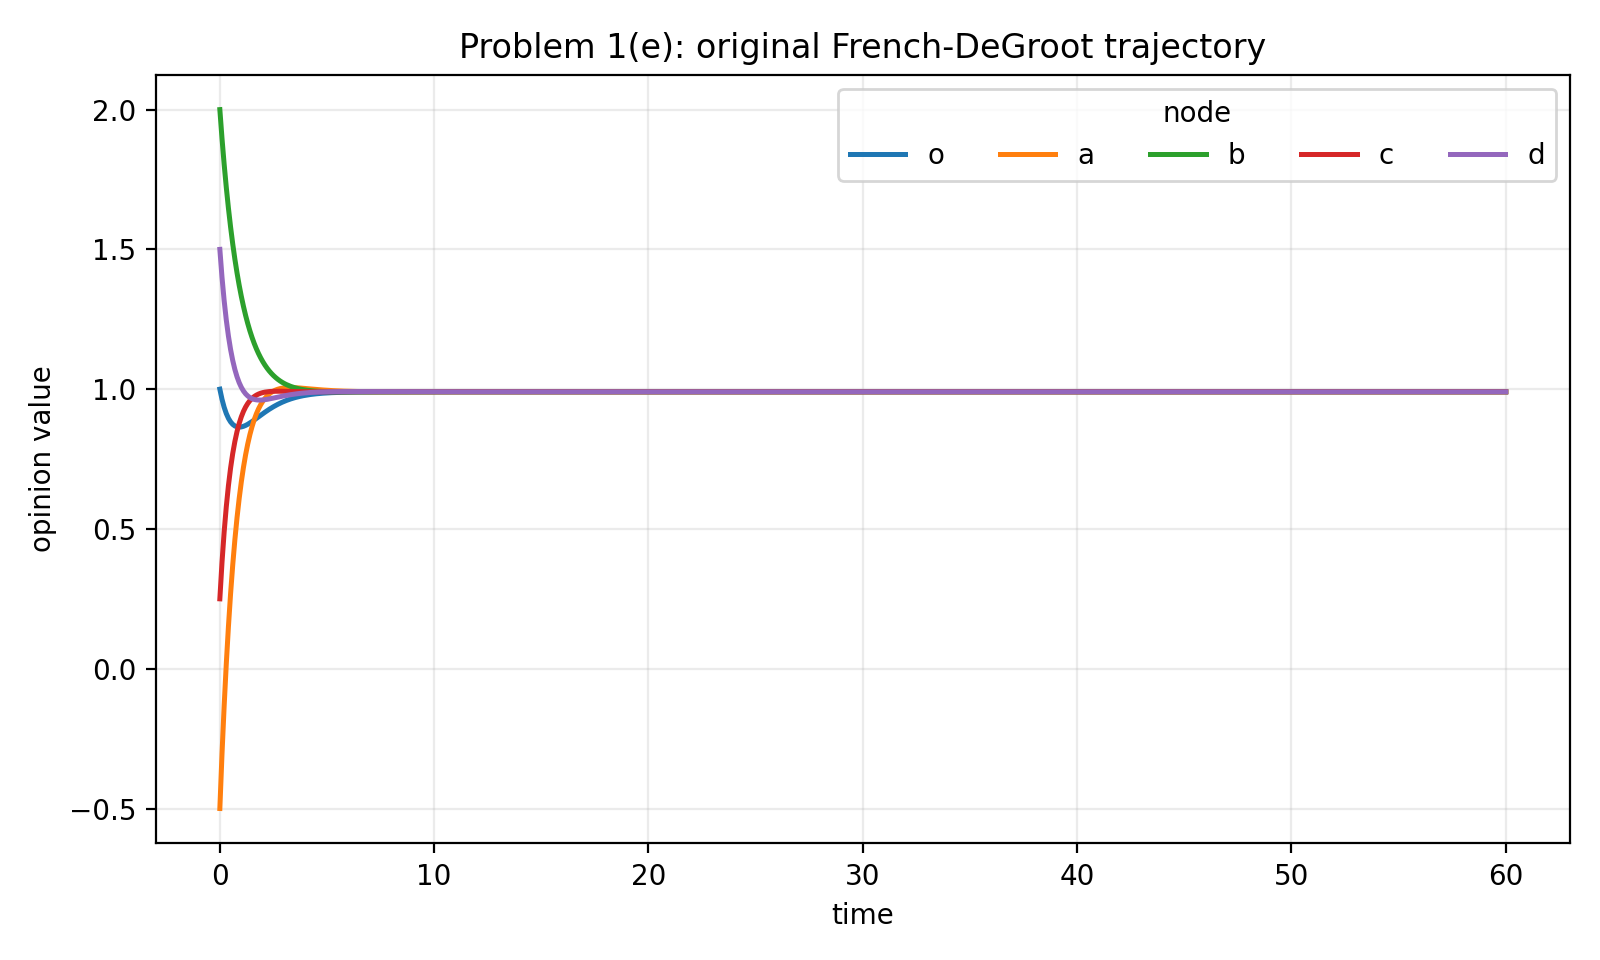
\includegraphics[width=0.85\linewidth]{../figures/problem1_fdg_original_trajectory.png}
    \caption{Continuous-time French-DeGroot trajectory on the original graph.}
    \label{fig:p1-fdg-original}
\end{figure}

The graph has one strongly connected component, namely
$\{o,a,b,c,d\}$, which is also the only sink strongly connected component.
Therefore every node can influence the unique sink component and the dynamics
converges to consensus for every initial condition. The consensus value has the
form
\[
    x^* = \sum_i \pi_i x_i(0),
\]
where $\pi$ is the normalized left nullvector associated with the zero
eigenvalue of $L$. For the original graph,
\[
\pi =
(0.21739130434782614,\,
0.14906832298136644,\,
0.26086956521739135,\,
0.18633540372670807,\,
0.186335403726708),
\]
again in the order $[o,a,b,c,d]$. For the plotted initial condition, the
consensus value is $0.990683229814$.

\subsection*{Part (f): variance of the consensus value}

The random initial condition has independent entries $x_i(0)=\xi_i$ with
\[
\operatorname{Var}(\xi_o)=1,\quad
\operatorname{Var}(\xi_a)=2,\quad
\operatorname{Var}(\xi_b)=2,\quad
\operatorname{Var}(\xi_c)=2,\quad
\operatorname{Var}(\xi_d)=1.
\]
Since $x^*=\sum_i \pi_i x_i(0)$, independence gives
\[
    \operatorname{Var}(x^*) =
    \sum_i \pi_i^2 \operatorname{Var}(x_i(0)).
\]
Using the consensus vector above, the theoretical variance is
\[
    \operatorname{Var}(x^*) = 0.33197.
\]
For the numerical comparison, I sampled independent centred Gaussian variables
with the prescribed variances, namely
$\xi_o,\xi_d\sim\mathcal{N}(0,1)$ and
$\xi_a,\xi_b,\xi_c\sim\mathcal{N}(0,2)$.
The theoretical variance depends only on independence and on these variances,
not on Gaussianity.
The Monte Carlo estimate, using 50000 independent samples with seed 20260617,
was $0.33128$, with sample mean $-0.00270$. The difference from
the theoretical variance was $-0.000692$, or relative error
$-0.00209$.

\begin{figure}[htbp]
    \centering
    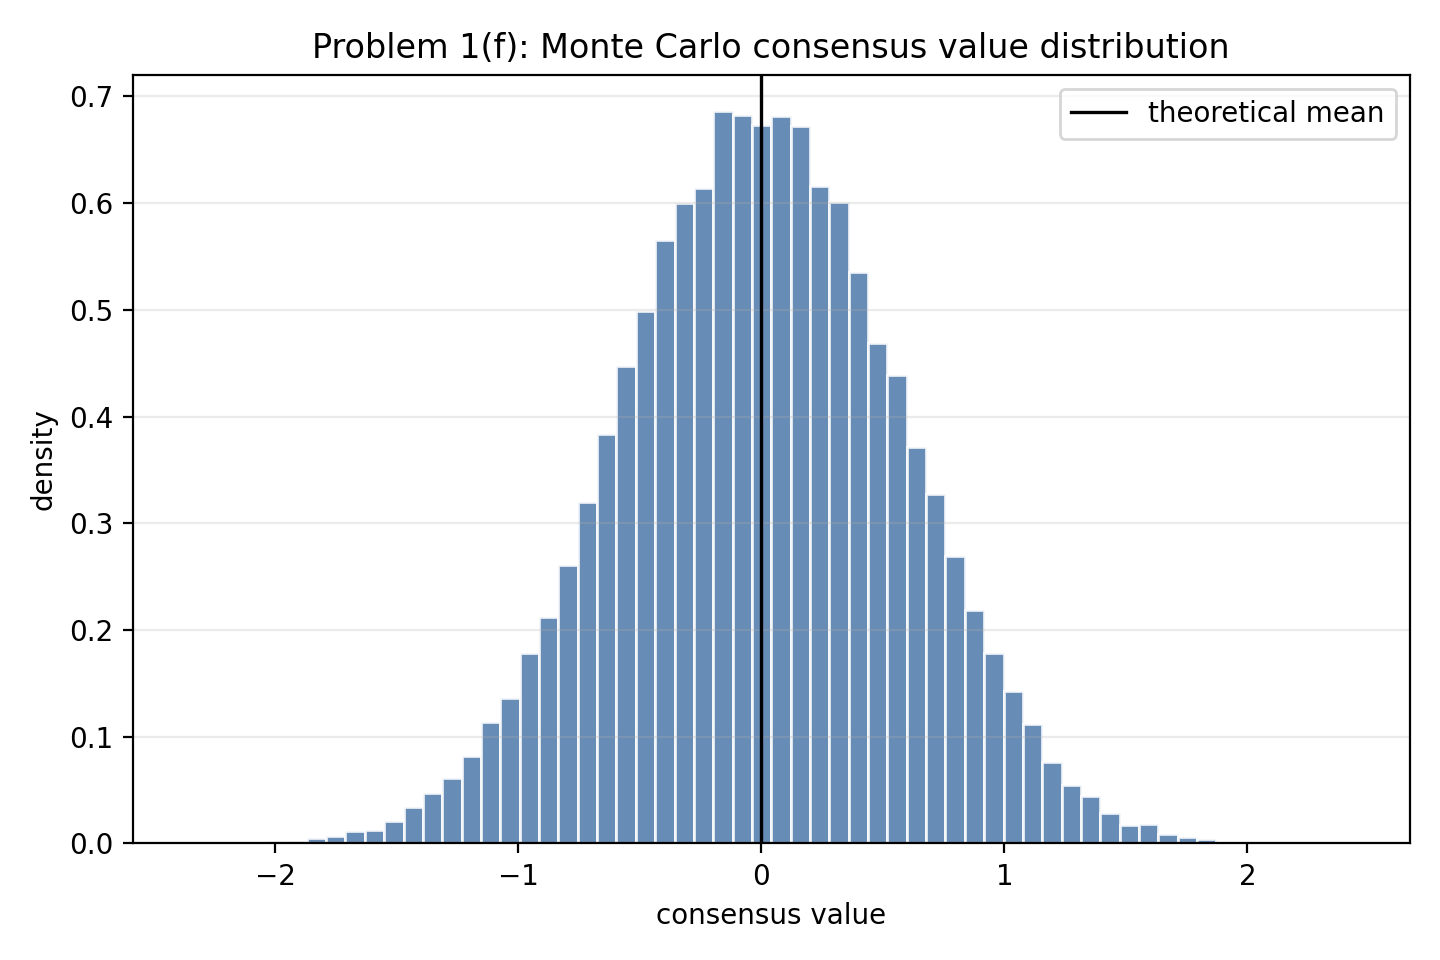
\includegraphics[width=0.80\linewidth]{../figures/problem1_consensus_value_histogram.png}
    \caption{Monte Carlo histogram of the consensus value for the random
    Gaussian initial condition in Part~(f), comparing the empirical consensus
    distribution with the theoretical variance.}
    \label{fig:p1-consensus-hist}
\end{figure}

Figure~\ref{fig:p1-consensus-hist} shows the empirical distribution of the
consensus value.

\subsection*{Part (g): removing $(d,a)$, $(d,c)$, $(a,c)$, and $(b,c)$}

For this modification, the entries $\Lambda_{d a}$, $\Lambda_{d c}$,
$\Lambda_{a c}$, and $\Lambda_{b c}$ are set to zero, using the row-source and
column-destination convention. The strongly connected components are
\[
    \{o,a,b\}, \qquad \{c\}, \qquad \{d\}.
\]
The sink strongly connected components are $\{o,a,b\}$ and $\{d\}$. Since there
are two sink components, the dynamics does not converge to a global consensus
for every initial condition.

For the representative initial condition
\[
    x(0) = (0,\,3,\,-1,\,2,\,5),
\]
the computed asymptotic state is approximately
\[
    (0.1463,\;
    0.1463,\;
    0.1463,\;
    3.3821,\;
    5.0).
\]
Thus nodes in the sink component $\{o,a,b\}$ reach one limiting value, node $d$
keeps its own sink value, and the transient node $c$ converges to a value
determined by the sink components reachable from it and by the initial
condition.

More explicitly, the component $\{o,a,b\}$ is closed and reaches its own
internal consensus value $z_{oab}$, while node~$d$ is an isolated sink and
keeps $x_d(0)$.  The transient node~$c$ listens to both $b$ (rate~$1/3$)
and $d$ (rate~$2/3$), so its limiting value is a weighted combination of the
sink values reachable from~$c$.  For the reported initial condition,
\[
x_c^\infty
=
\tfrac{1}{3}\,z_{oab}
+
\tfrac{2}{3}\,x_d(0)
=
\tfrac{1}{3}(0.1463)
+
\tfrac{2}{3}(5)
=
3.3821.
\]

\begin{figure}[htbp]
    \centering
    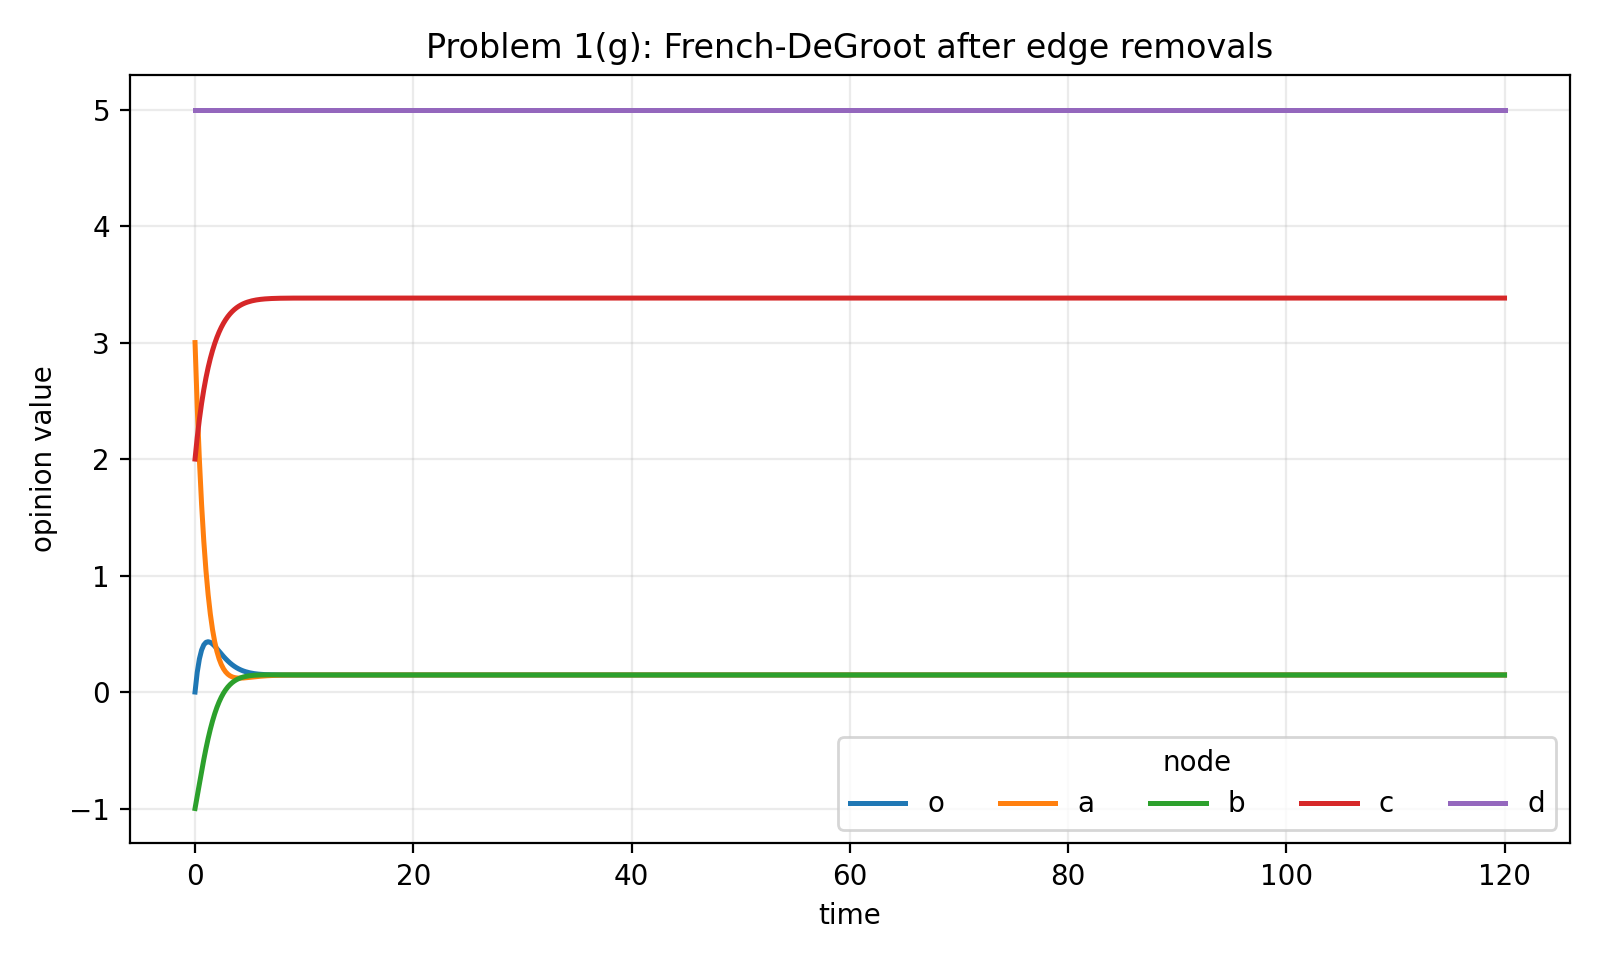
\includegraphics[width=0.85\linewidth]{../figures/problem1_fdg_removed_edges_g.png}
    \caption{French-DeGroot trajectory after removing $(d,a)$, $(d,c)$,
    $(a,c)$, and $(b,c)$.}
    \label{fig:p1-removed-g}
\end{figure}

Figure~\ref{fig:p1-removed-g} illustrates the non-consensus limiting behavior.

\subsection*{Part (h): removing $(b,o)$ and $(d,a)$}

For this modification, the entries $\Lambda_{b o}$ and $\Lambda_{d a}$ are set
to zero. The strongly connected components are
\[
    \{o\}, \qquad \{a\}, \qquad \{b,c,d\}.
\]
The only sink strongly connected component is $\{b,c,d\}$, and it is reachable
from all nodes. Therefore the continuous-time French-DeGroot dynamics converges
to a global consensus for every initial condition, but the consensus value is
determined by the initial values in the sink component through its left
eigenvector.

For the modified graph, the normalised left eigenvector associated with the
unique sink SCC $\{b,c,d\}$, extended by zeros on the transient
nodes~$o$ and~$a$, is
\[
\pi^{(h)}=(0,\,0,\,1/4,\,1/4,\,1/2).
\]
Hence, for every initial condition,
\[
\lim_{t\to\infty}x(t)
=
\left(
\tfrac{1}{4}\,x_b(0)
+
\tfrac{1}{4}\,x_c(0)
+
\tfrac{1}{2}\,x_d(0)
\right)\mathbf{1}.
\]
Therefore the initial opinions of~$o$ and~$a$ do not affect the final
consensus value; they only affect the transient trajectory.

Two representative simulations are shown in Figures~\ref{fig:p1-removed-h1}
and~\ref{fig:p1-removed-h2}. For
\[
    x(0) = (0,\,3,\,-1,\,2,\,5),
\]
the consensus value is
$\frac{1}{4}(-1)+\frac{1}{4}(2)+\frac{1}{2}(5)=2.75$,
and the asymptotic state is $(2.75,2.75,2.75,2.75,2.75)$. For
\[
    x(0) = (10,\,-4,\,1,\,-2,\,0.5),
\]
the consensus value is
$\frac{1}{4}(1)+\frac{1}{4}(-2)+\frac{1}{2}(0.5)=0$,
and the asymptotic state is zero at all nodes, up to numerical
roundoff. These two cases show that the graph structure guarantees consensus,
while the actual consensus value still depends on $x(0)$.

\begin{figure}[htbp]
    \centering
    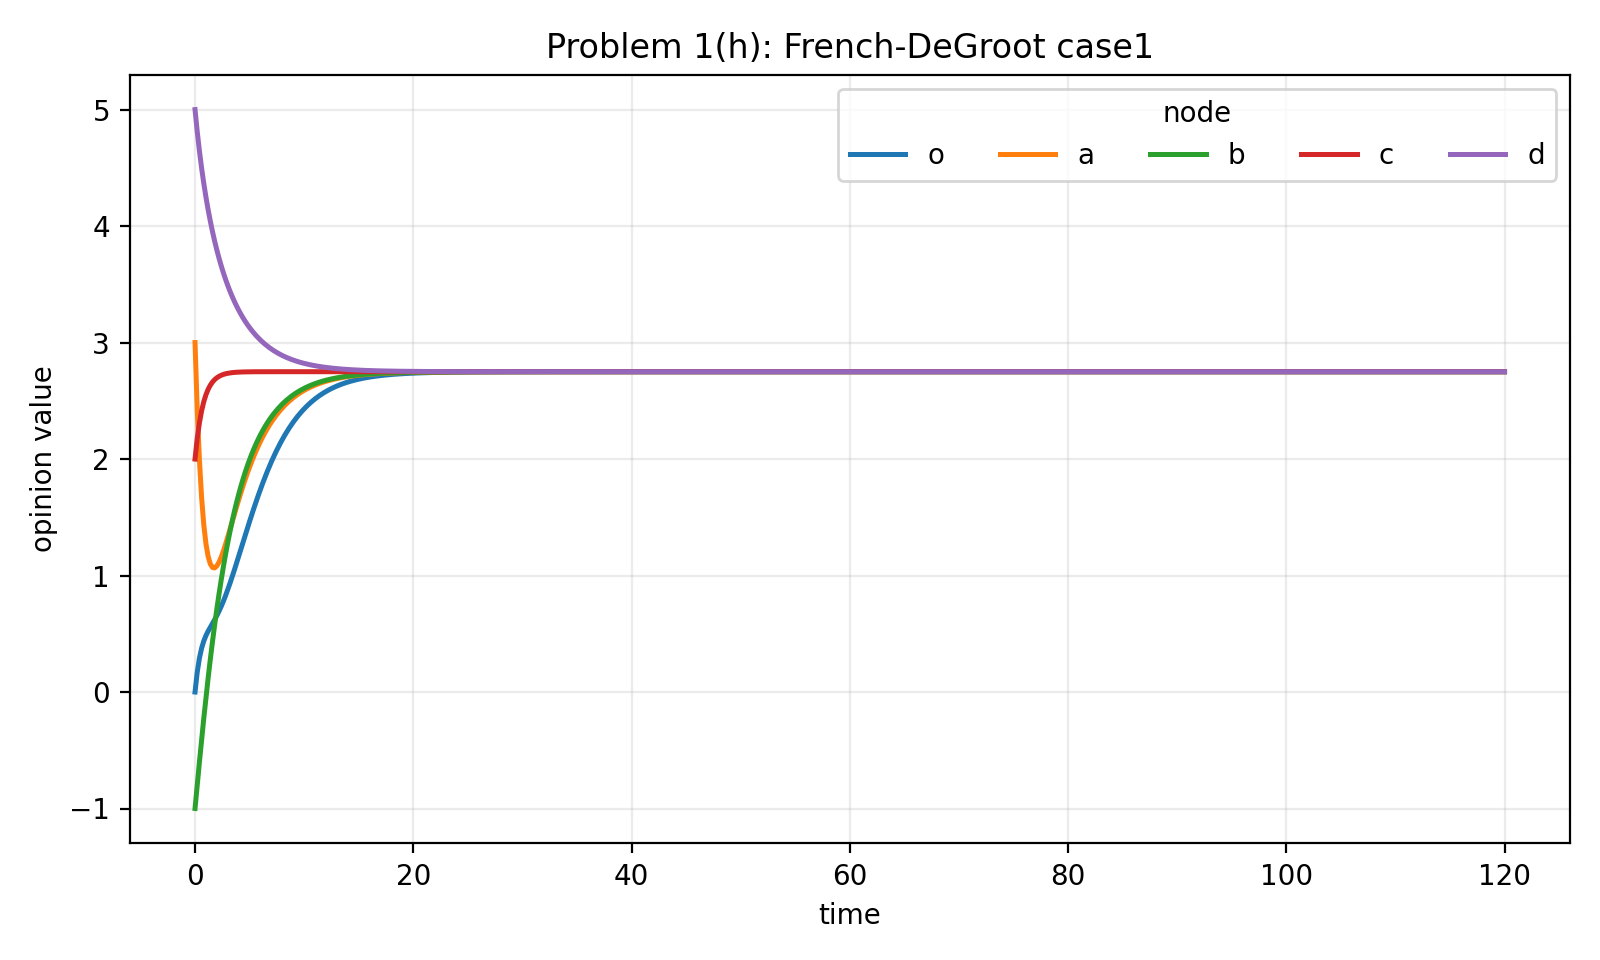
\includegraphics[width=0.85\linewidth]{../figures/problem1_fdg_removed_edges_h_case1.png}
    \caption{French-DeGroot trajectory after removing $(b,o)$ and $(d,a)$,
    first representative initial condition.}
    \label{fig:p1-removed-h1}
\end{figure}

\begin{figure}[htbp]
    \centering
    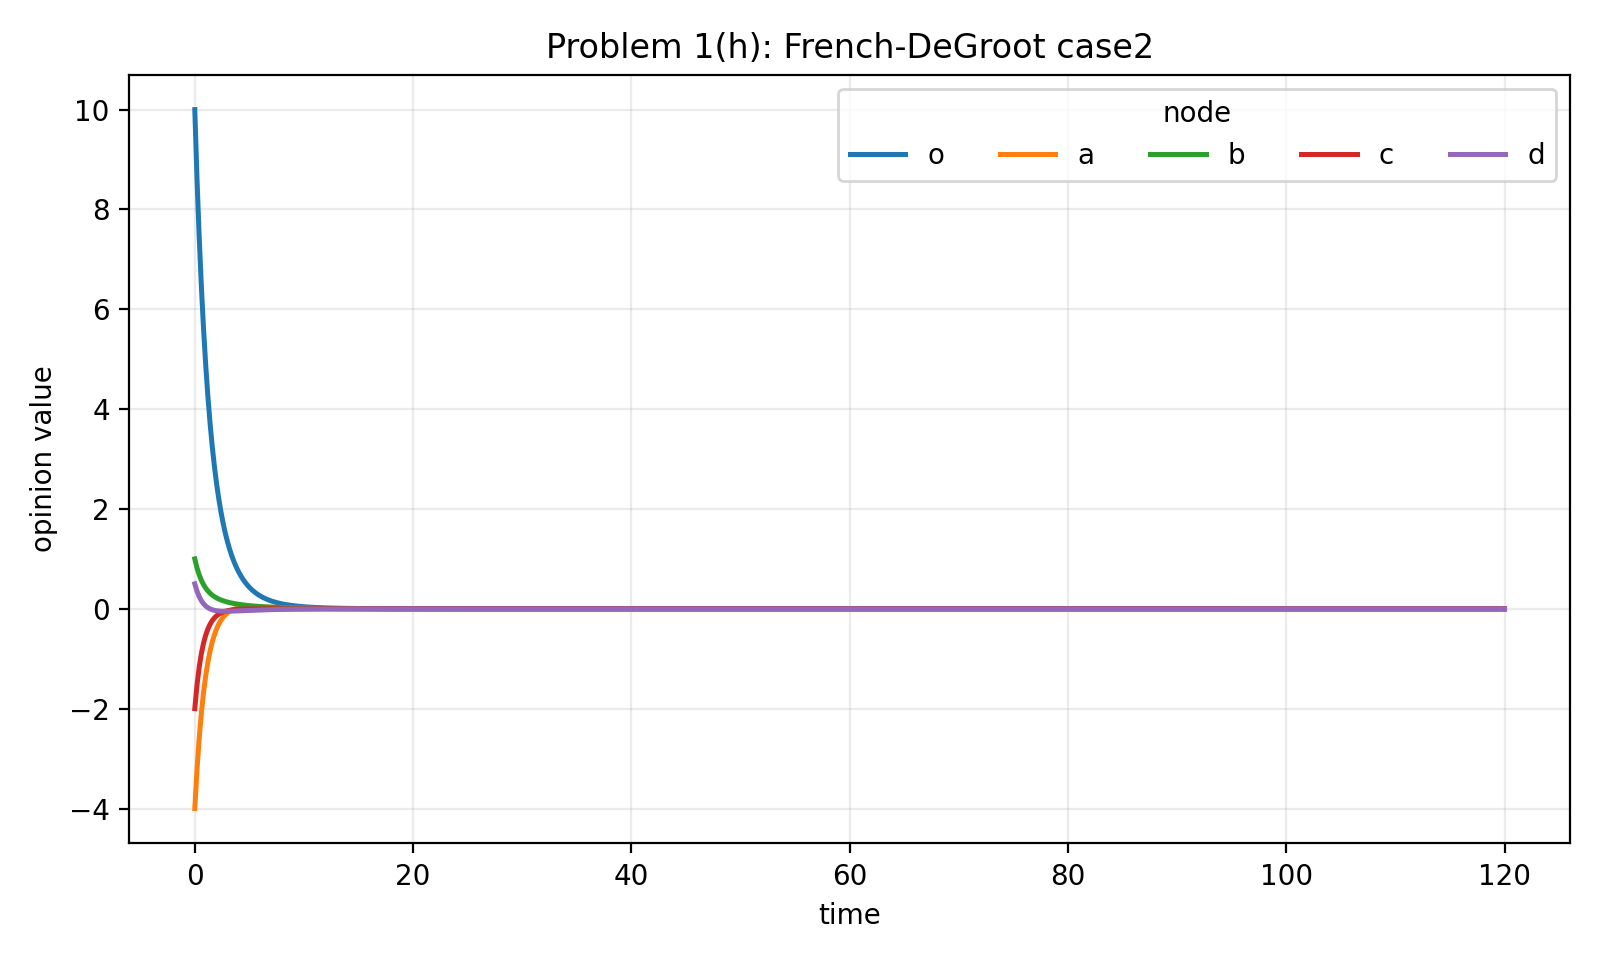
\includegraphics[width=0.85\linewidth]{../figures/problem1_fdg_removed_edges_h_case2.png}
    \caption{French-DeGroot trajectory after removing $(b,o)$ and $(d,a)$,
    second representative initial condition.}
    \label{fig:p1-removed-h2}
\end{figure}

\section{Problem 2 --- Many-particle continuous-time random walks}

The many-particle model uses the same closed network as Problem 1, with node
order
\[
    [o,a,b,c,d].
\]
There are $N=100$ particles. For one particle, the total departure-rate vector
is
\[
    \omega = \Lambda \mathbf{1},
\]
and the continuous-time generator is
\[
    Q = \Lambda - \operatorname{diag}(\omega).
\]
After a departure from node $i$, the destination is sampled from the embedded
jump matrix
\[
    P_{\mathrm{jump}}
    = \operatorname{diag}(\omega)^{-1}\Lambda,
    \qquad
    (P_{\mathrm{jump}})_{ij} = \frac{\Lambda_{ij}}{\omega_i}.
\]
This is the transition matrix of the jump chain observed only at actual jump
times. It is therefore different from a uniformized discrete-time transition
matrix, which would usually include self-loop probabilities. This distinction
matters because the node-count simulation below samples only actual CTMC
departure events; it does not insert artificial self-loop events.

There are two equivalent perspectives. In the particle perspective, each of the
$100$ particles is followed as an independent copy of the single-particle CTMC
from Problem 1. In the node perspective, the state is the vector of occupation
counts
\[
    N(t) = (N_o(t),N_a(t),N_b(t),N_c(t),N_d(t)),
\]
where $N_i(t)$ is the number of particles at node $i$ at time $t$.

\subsection*{Part (a): particle perspective}

For the particle-perspective simulation, all $N=100$ particles start in node
$a$, and each particle follows the same CTMC used in Problem 1. The return-time
convention is also the same as in Problem 1: the initial holding time in node
$a$ is included, and the stopping time is the next entrance to $a$ after the
particle has left.

The simulation used 2000 Monte Carlo repetitions with seed 20260624, giving
$200000$ total particle return times. The estimated average return time to node
$a$ was
\[
    \widehat{\mathbb{E}}_a[T_a^+] = 6.70478013087,
\]
with standard error $0.0107350702469$ across the run-level particle averages
and 95 percent confidence interval
$[6.68373939319,\,6.72582086855]$.

For comparison, Problem 1(a) gave simulated mean $6.69375284456$ with standard
error $0.0155366695236$, while the theoretical value from Problem 1(b) was
$6.70833333333$. The many-particle estimate differs from the Problem 1
simulation by $0.0110272863097$ and from the theoretical value by
$-0.00355320246031$. The agreement is expected because, from the particle
perspective, the experiment is just many independent repetitions of the same
single-particle CTMC.

\subsection*{Part (b): node perspective}

In the node perspective, the Markov state records only the number of particles
at each node. The initial condition is
\[
    N(0) = (0,100,0,0,0),
\]
in the node order $[o,a,b,c,d]$. If there are $n_i(t)$ particles at node $i$,
then departures from node $i$ occur at total rate $n_i(t)\omega_i$. Conditional
on such a departure, the destination is sampled according to the $i$th row of
$P_{\mathrm{jump}}$, and one particle count is moved from node $i$ to the
destination node. The simulation horizon was $T=60$, using 5000 Monte Carlo
runs with seed 20260625.

The average final counts at $T=60$ were
\[
\begin{array}{c|ccccc}
\text{node} & o & a & b & c & d\\
\hline
\text{average count} & 21.7254 & 14.9592 & 25.9910 & 18.6466 & 18.6778
\end{array}
\]
The full trajectory of the average node counts is shown in
Figure~\ref{fig:p2-node-counts}.

\begin{figure}[htbp]
    \centering
    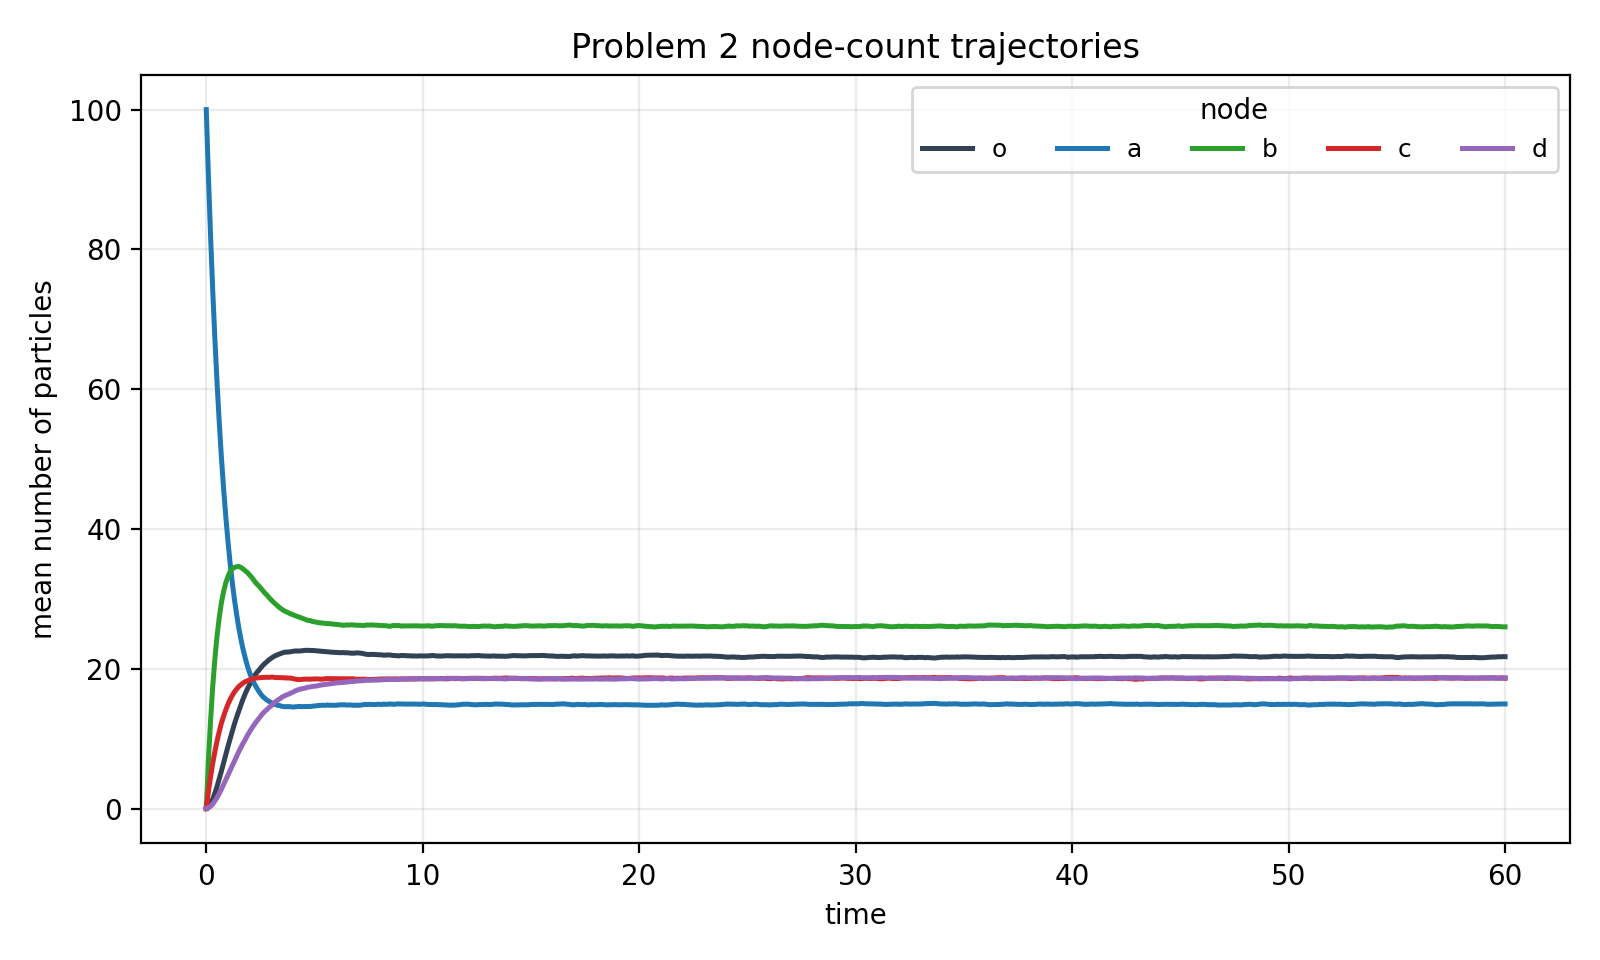
\includegraphics[width=0.85\linewidth]{../figures/problem2_node_counts_over_time.png}
    \caption{Average node counts over time for $N=100$ particles, with all
    particles initially in node $a$ and simulation horizon $T=60$. Each curve
    represents the count of particles at one node as a function of time.}
    \label{fig:p2-node-counts}
\end{figure}

\subsection*{Stationary distribution comparison}

Let $\pi$ denote the stationary distribution of the single-particle CTMC. It is
defined by
\[
    \pi Q = 0, \qquad \sum_i \pi_i = 1.
\]
For $N$ independent particles at stationarity, the expected node-count vector
is $N\pi$. The comparison between the simulated average final counts at
$T=60$ and $100\pi$ is
\[
\begin{array}{c|ccccc}
\text{node} & o & a & b & c & d\\
\hline
\text{average count at }T=60
& 21.7254 & 14.9592 & 25.9910 & 18.6466 & 18.6778\\
100\pi
& 21.7391304348 & 14.9068322981 & 26.0869565217
& 18.6335403727 & 18.6335403727
\end{array}
\]
The comparison is visualized in
Figure~\ref{fig:p2-stationary-comparison}. The simulated final averages are
close to $100\pi$, with small discrepancies due to the finite time horizon
$T=60$ and Monte Carlo sampling error.

\begin{figure}[htbp]
    \centering
    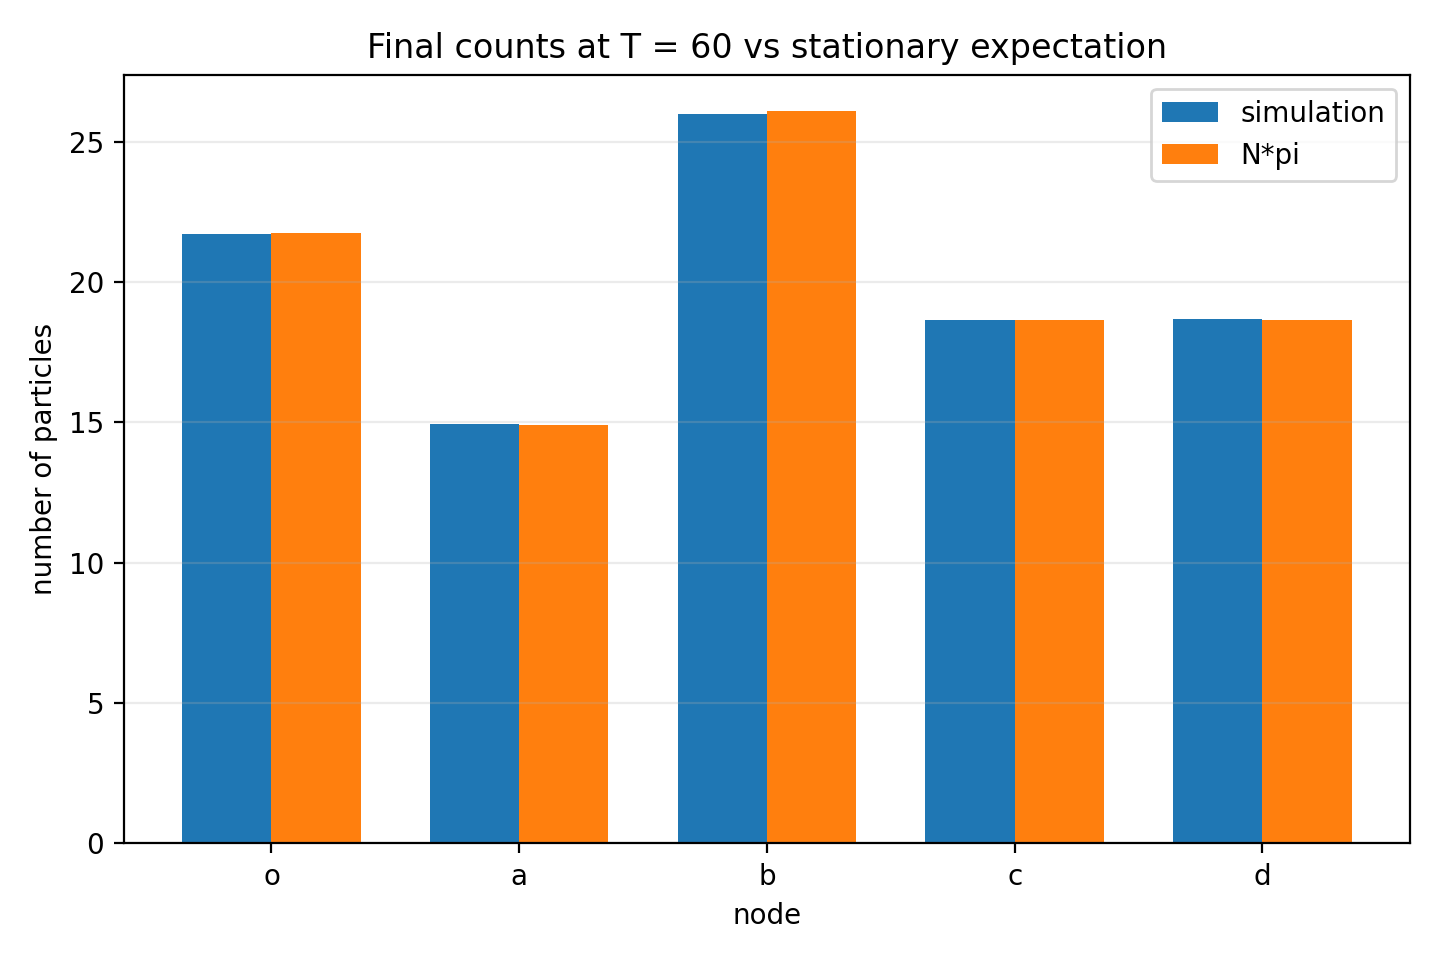
\includegraphics[width=0.80\linewidth]{../figures/problem2_stationary_distribution_comparison.png}
    \caption{Comparison of the average final node counts at $T=60$ with the
    stationary expected counts $N\pi$ for $N=100$ particles.}
    \label{fig:p2-stationary-comparison}
\end{figure}

\section{Problem 3 --- Open network with proportional and fixed service rates}

\subsection*{Open-network model}

The node order is again
\[
    [o,a,b,c,d].
\]
For the open network I use
\[
\Lambda_{\mathrm{open}} =
\begin{pmatrix}
0 & 1 & 1 & 0 & 0\\
0 & 0 & 1/4 & 1/4 & 2/4\\
0 & 0 & 0 & 1 & 0\\
0 & 0 & 0 & 0 & 1\\
0 & 0 & 0 & 0 & 0
\end{pmatrix}.
\]
The matrix orientation is row-source and column-destination:
$(\Lambda_{\mathrm{open}})_{ij}$ is the rate from node $i$ to node $j$.
External arrivals enter node $o$ according to a Poisson process of rate
$\lambda$. Let
\[
    N(t) = (N_o(t),N_a(t),N_b(t),N_c(t),N_d(t))
\]
be the vector of particle counts. The service-rate vector is
\[
    \omega = \Lambda_{\mathrm{open}}\mathbf{1},
\]
with the special assignment $\omega_d=7/4$. Thus the values used in the
simulation are
\[
    \omega = (2,1,1,1,7/4).
\]
For nodes $o,a,b,c$, a service event at a nonempty node forwards one particle
according to the normalized outgoing rates in the corresponding row of
$\Lambda_{\mathrm{open}}$. Node $d$ is the exit node: when the clock at node
$d$ ticks and $N_d(t)>0$, one particle leaves the system.

\subsection*{Part (a): proportional-rate scenario}

In the proportional-rate model, node $i$ forwards particles at total rate
$\omega_i N_i(t)$. The simulation is an event-based continuous-time simulation:
external arrivals, node service events, and removals at $d$ are sampled from
their current exponential clocks, and the count vector is recorded on a fixed
time grid. Figure~\ref{fig:p3-proportional-counts} shows a single sample path
with $\lambda=100$ and horizon $T=60$. At time $T=60$, the recorded counts are
\[
    (48,39,72,62,63),
\]
for a total of $284$ particles.

\begin{figure}[htbp]
    \centering
    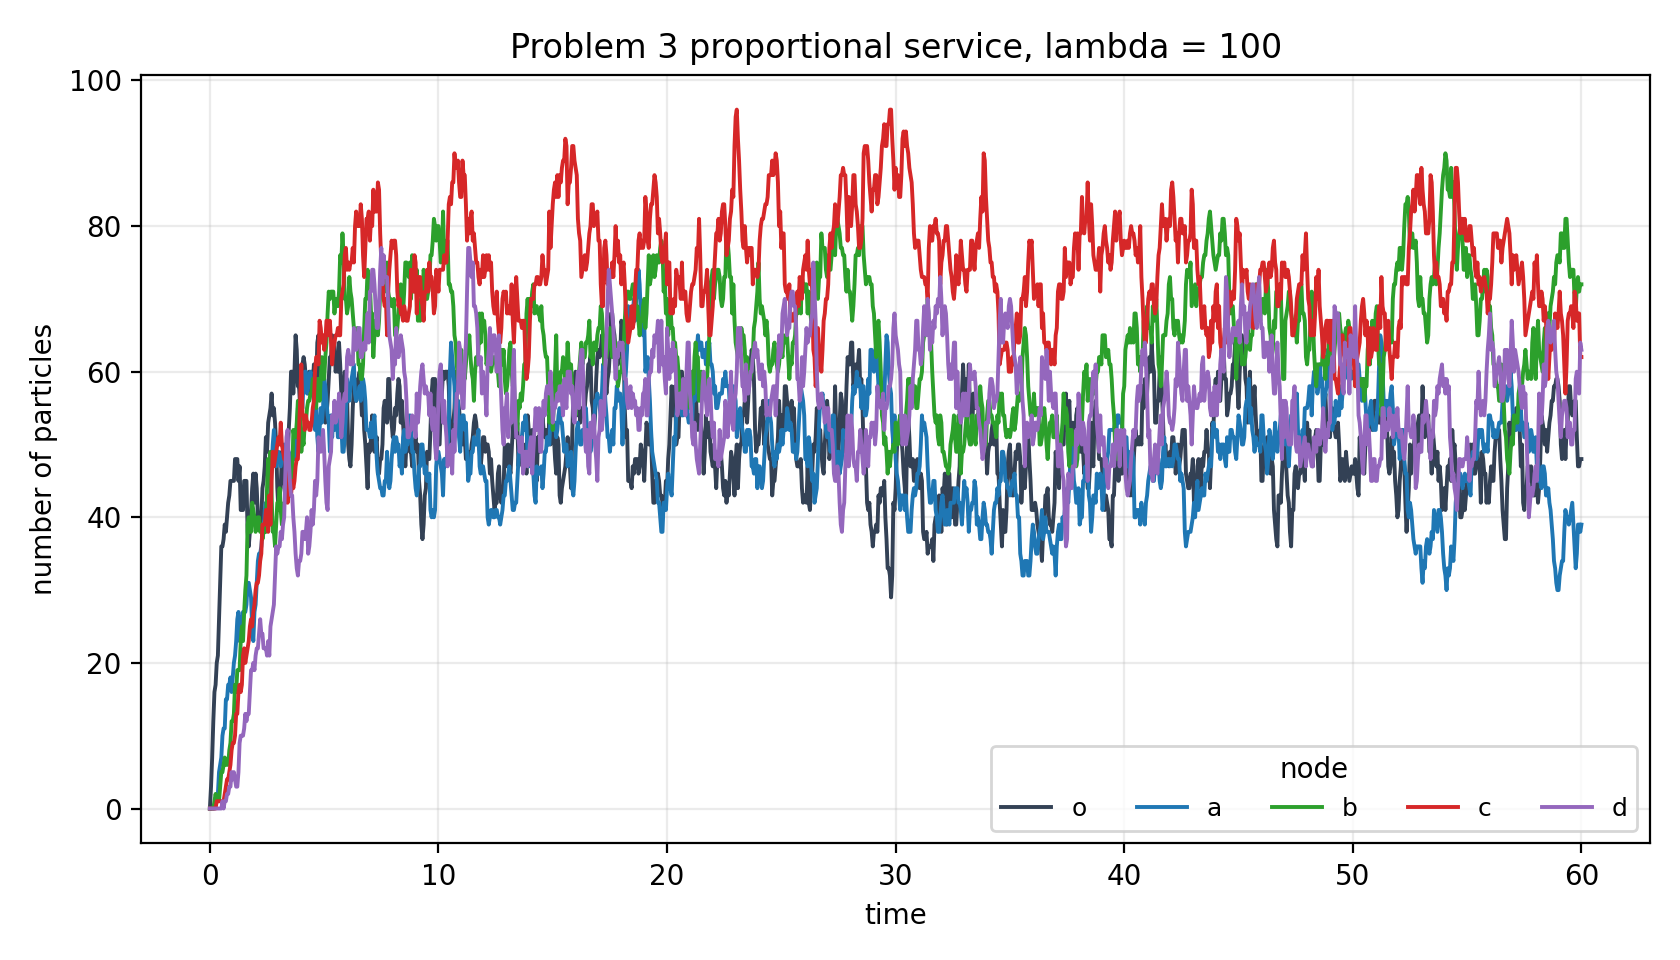
\includegraphics[width=0.85\linewidth]{../figures/problem3_proportional_lambda100_counts.png}
    \caption{Single sample path of open-network particle counts under
    proportional service with $\lambda=100$ and $T=60$.}
    \label{fig:p3-proportional-counts}
\end{figure}

The trajectory fluctuates around a finite population scale rather than showing
sustained linear growth. The theoretical reason is that proportional service
makes each node act like an infinite-server queue: as $N_i(t)$ grows, the
aggregate departure rate from node $i$ grows proportionally. The expected
single-particle remaining lifetimes from $(o,a,b,c,d)$ are
\[
    (2.9464,\;2.3214,\;2.5714,\;1.5714,\;
    0.5714),
\]
so any finite external input rate gives a finite expected population.
Equivalently, by Little's-law intuition, the expected total number of
particles in the system is proportional to
$\lambda\,\mathbb{E}_o[T_{\mathrm{exit}}]$.  Since
$\mathbb{E}_o[T_{\mathrm{exit}}]=2.9464<\infty$, this expectation is finite
for every finite~$\lambda$.  Thus the proportional-rate model has no finite
theoretical blow-up threshold; increasing~$\lambda$ increases the typical
population size approximately linearly, but does not create instability in the
fixed-capacity sense.
Therefore there is no finite theoretical upper bound on the stable input rate
for this proportional-rate model. The stability scan below should be read as
implementation evidence for the finite input rates tested, not as the
theoretical proof of stability.

The stability scan in Figure~\ref{fig:p3-proportional-scan} tested
$\lambda=10,50,100,200,500$ over horizon $120$ with two replicates per value.
The implementation classified a proportional run as blow-up if the mean fitted
slope of the total population over the second half of the horizon exceeded
$0.05\lambda$. None of the tested values met this criterion; the largest tested
input rate, $\lambda=500$, was classified as stable by the scan, with mean
final total $1445.5$ and mean second-half slope $-0.571370967742$.

\begin{figure}[htbp]
    \centering
    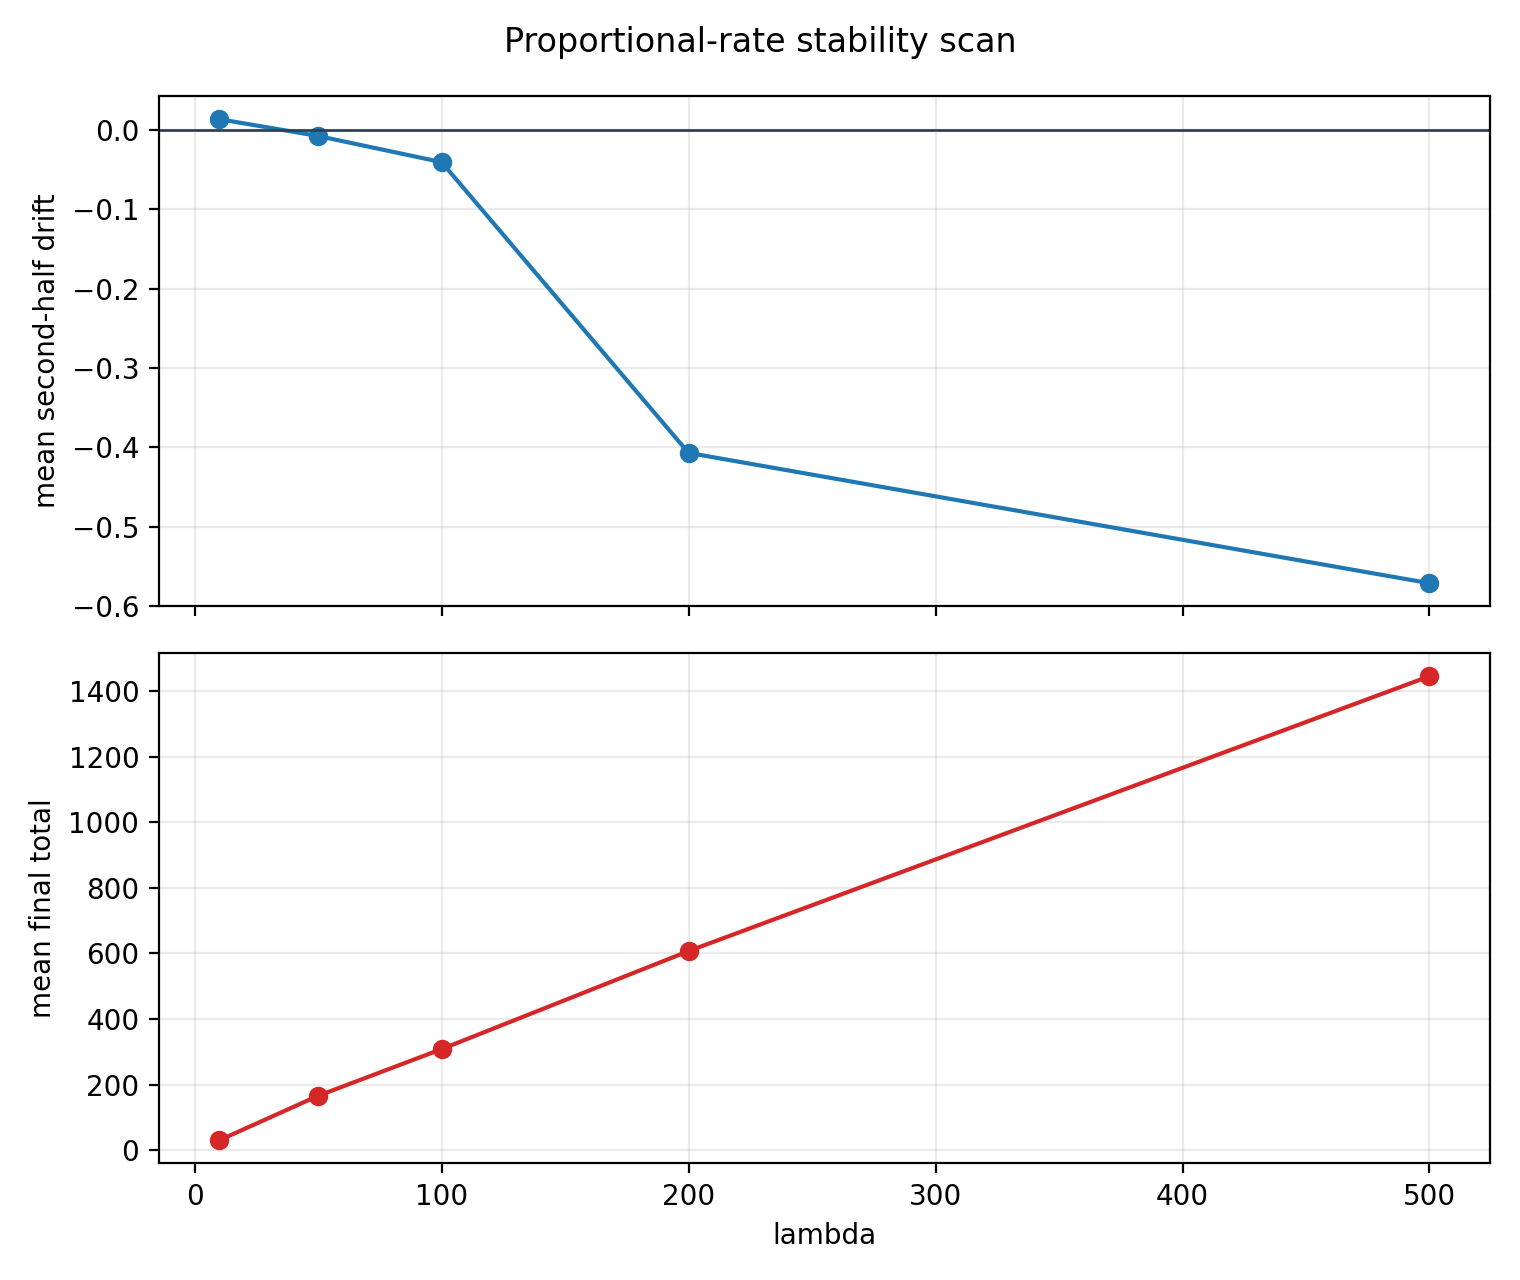
\includegraphics[width=0.85\linewidth]{../figures/problem3_proportional_stability_scan.png}
    \caption{Stability scan for proportional service. Classification is based
    on the fitted second-half drift of total population, not only on visual
    inspection.}
    \label{fig:p3-proportional-scan}
\end{figure}

\subsection*{Part (b): fixed-rate scenario}

In the fixed-rate model, node $i$ has a service clock of fixed rate
$\omega_i$, independent of $N_i(t)$. If the clock of an empty node ticks,
nothing is moved. If the node is nonempty, one particle is forwarded using the
same routing probabilities as above, except that a nonempty service event at
node $d$ removes one particle from the system.

Figure~\ref{fig:p3-fixed-counts} shows a single sample path of the fixed-rate
simulation with $\lambda=2$ and $T=6000$. At time $T=6000$, the recorded
counts are
\[
    (233,15,1240,1577,6),
\]
for a total of $3071$ particles. The qualitative behavior is different from
the proportional case: the population grows because service capacity does not
increase when queues become large.

\begin{figure}[htbp]
    \centering
    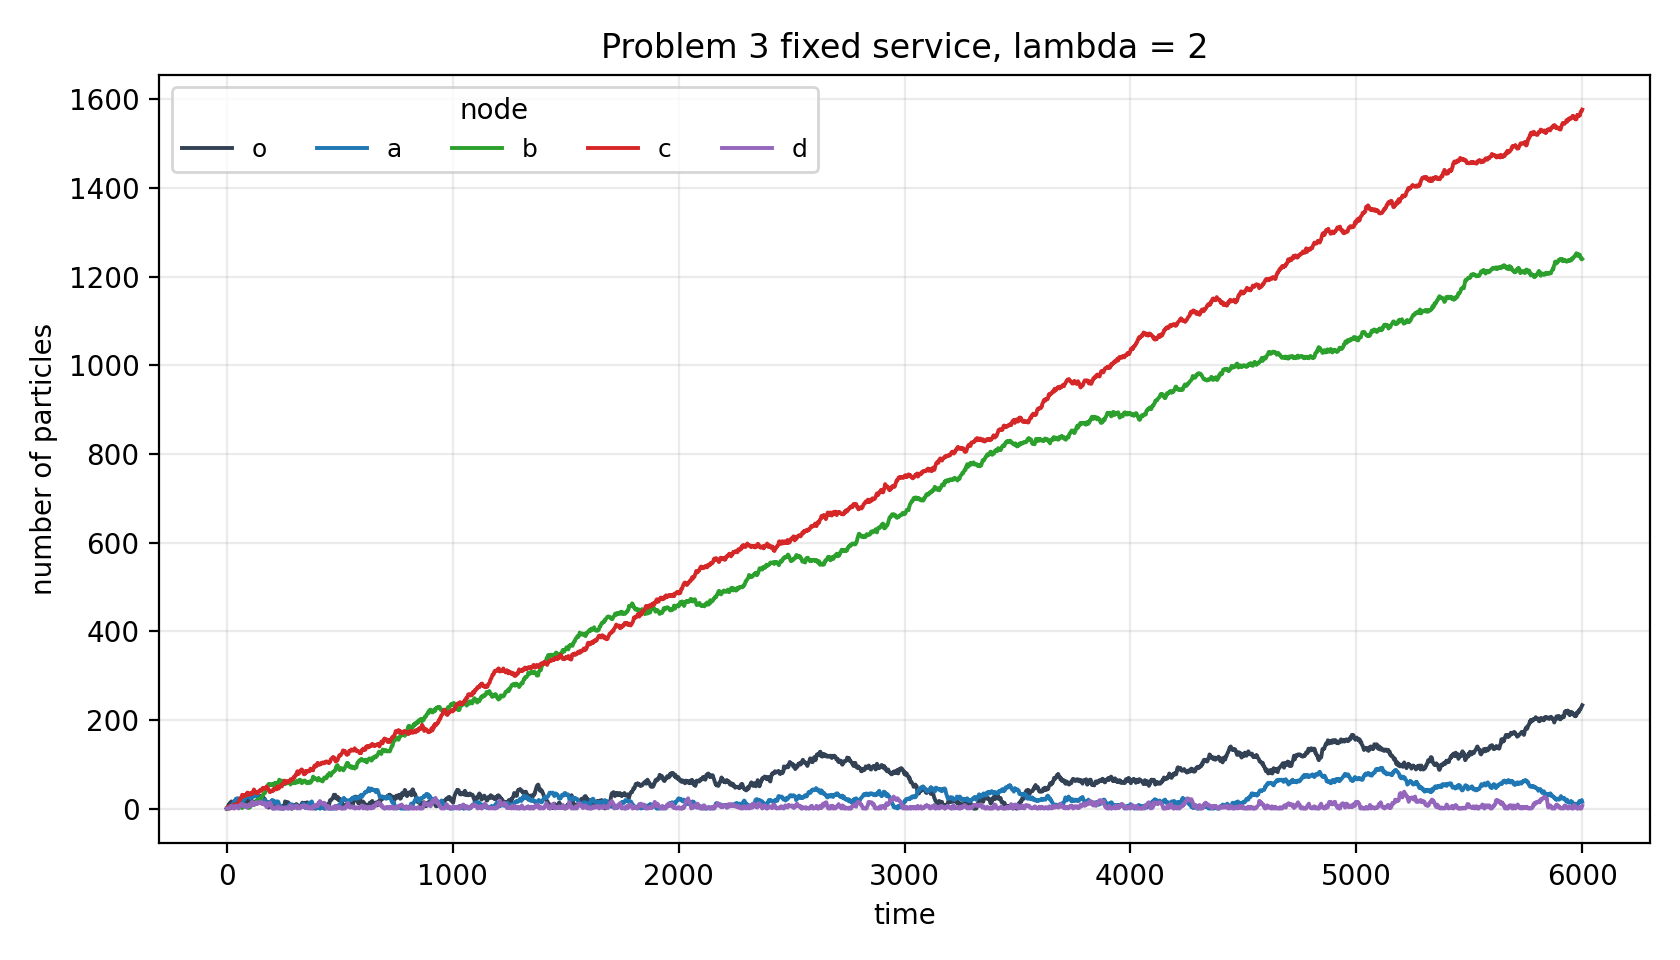
\includegraphics[width=0.85\linewidth]{../figures/problem3_fixed_lambda2_counts.png}
    \caption{Single sample path of open-network particle counts under fixed
    service with $\lambda=2$ and $T=6000$.}
    \label{fig:p3-fixed-counts}
\end{figure}

The bottleneck calculation uses the traffic load induced by one unit of
external arrival rate. The loads per unit $\lambda$ are
\[
    (1,\;1/2,\;5/8,\;3/4,\;1),
\]
so the fixed-rate capacity by node is
\[
    (2,\;2,\;1.6,\;4/3,\;1.75).
\]
The bottleneck node is~$c$, giving the critical threshold
\[
\lambda_c=\frac{4}{3}.
\]
The fixed-rate network is stable for $\lambda<4/3$ and unstable for
$\lambda\ge 4/3$.  Therefore $4/3$ is the supremum of sustainable input rates,
not a stable operating point itself.

The stability scan in Figure~\ref{fig:p3-fixed-scan} tested
$\lambda=0.5,1,1.2,1.3,4/3,1.35,1.5,2$ over horizon $6000$ with three
replicates per value. The implementation classified a fixed-rate run as
blow-up if either the mean fitted slope of the total population over the second
half of the horizon exceeded $0.005$, or the mean final total exceeded $1000$.
The scan classified $\lambda=1.3$ as stable, with mean final total $27$ and
mean second-half slope $0.00343644707796$. It classified $\lambda=4/3$ as
blow-up, with mean final total $125.333333333$ and mean second-half slope
$0.017733066109$. For $\lambda=2$, the scan mean final total was
$3144.66666667$ and the mean second-half slope was $0.518004182642$.

\begin{figure}[htbp]
    \centering
    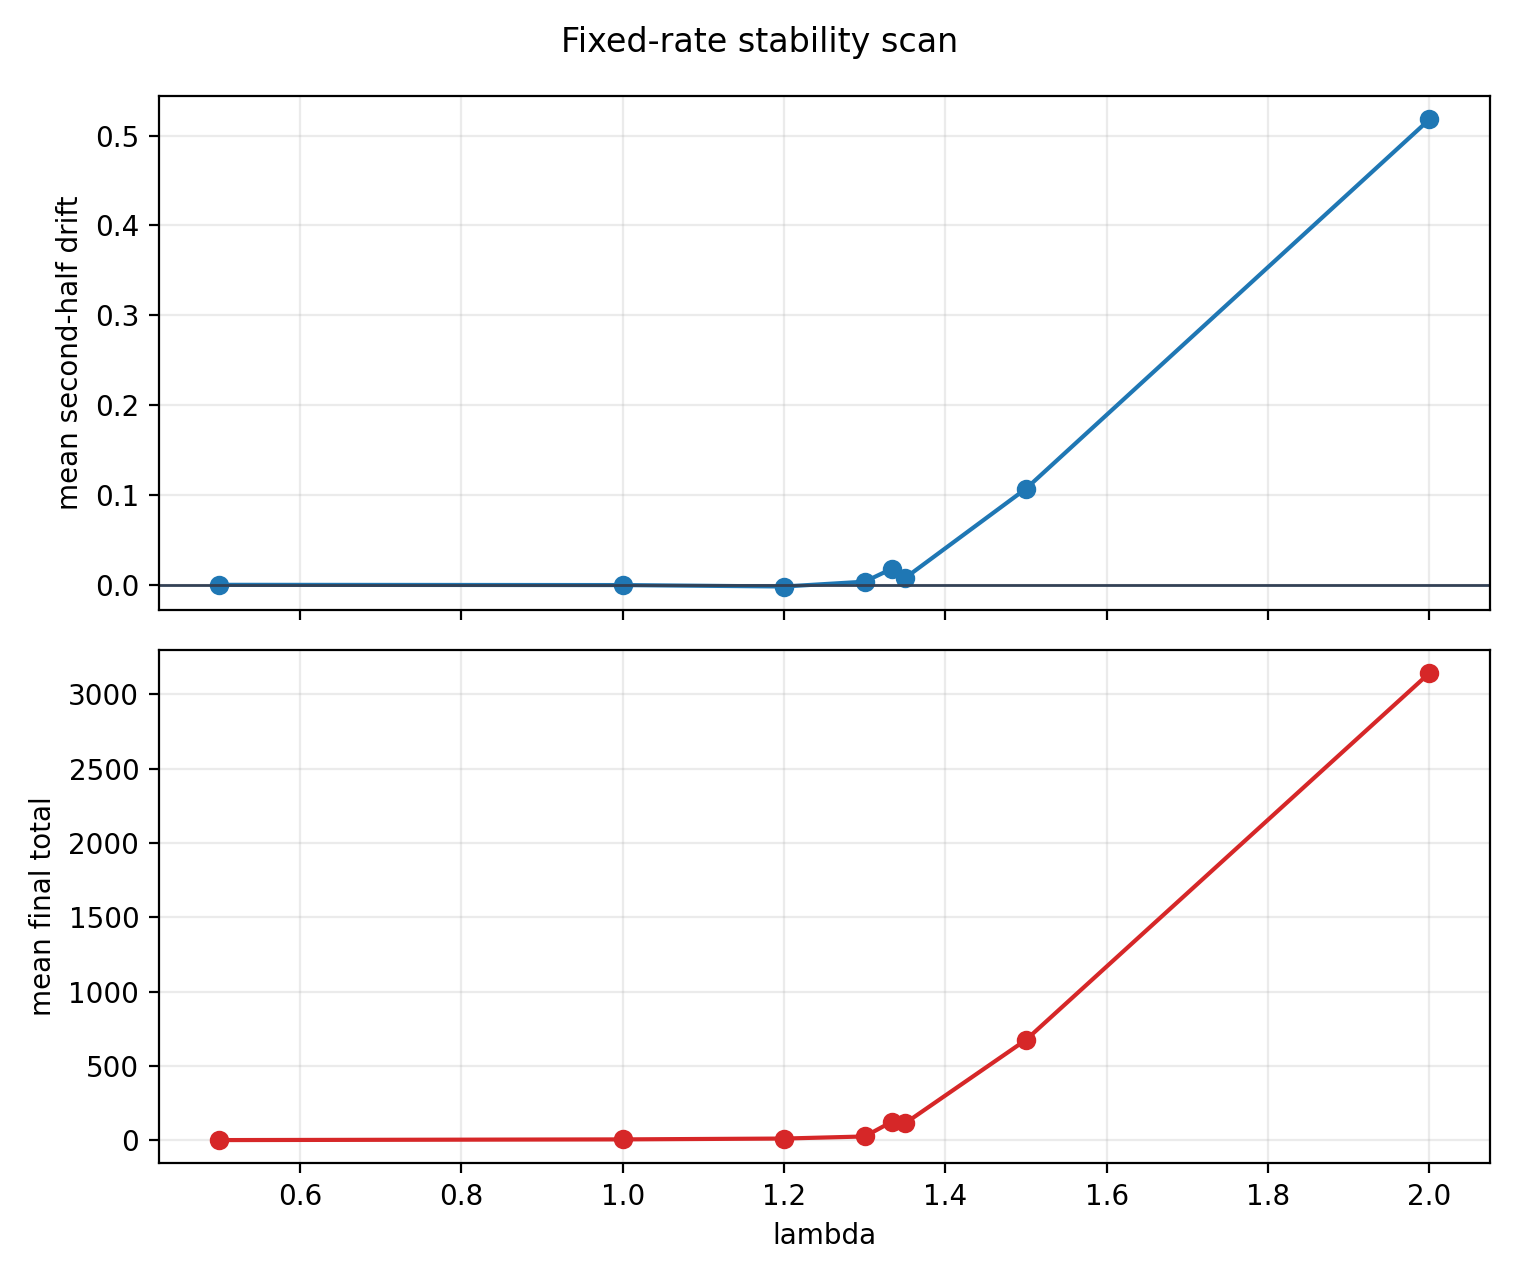
\includegraphics[width=0.85\linewidth]{../figures/problem3_fixed_stability_scan.png}
    \caption{Stability scan for fixed service. The threshold is determined
    from the second-half drift and final-total criteria together with the
    bottleneck capacity calculation.}
    \label{fig:p3-fixed-scan}
\end{figure}

\subsection*{Comparison}

The main distinction is that proportional service grows with the number of
particles in a node, while fixed service imposes hard service-capacity limits.
As a result, the proportional model remains stable for every finite input rate
in this network, whereas the fixed-rate model has a finite bottleneck
threshold at node $c$. In both cases, the plotted sample paths illustrate the
behavior, while the stability conclusion comes from the service-rate structure
and the replicated scan criterion described above.

\section{Conclusion}

In Problem 1, the single-particle CTMC simulations matched the theoretical
return and hitting times within Monte Carlo error. The French-DeGroot analysis
showed consensus on the original strongly connected graph, quantified the
variance of the random consensus value, and showed how removing edges can
either destroy global consensus or preserve it through a unique reachable sink
component.

In Problem 2, the particle-perspective simulation reproduced the same return
time behavior as the single-particle chain because the particles evolve
independently. The node-count simulation approached the stationary expected
counts $N\pi$, with the remaining differences attributable to the finite
horizon and Monte Carlo sampling.

In Problem 3, proportional service produced stable finite-population behavior
for the tested finite input rates because service capacity grows with the
number of particles. Fixed service produced a finite bottleneck threshold at
node $c$, and the simulation scan agreed with the theoretical distinction
between rates below the threshold and rates at or above it.

\section{Collaboration statement}

This work was completed individually. No collaboration was used beyond general
course material and standard references.

\end{document}
